\documentclass[titlepage, a4paper, 10pt, reqno, openany]{report}
%%%%%\usepackage{amscls}
\usepackage{amsfonts}
%%%%%\usepackage[brazil]{babel} %linguagem do documento
%%%%%\usepackage{babel}
%%%%%\usepackage[utf8]{inputenc} %reconhece acento e cedilha
\usepackage{amsmath}
\usepackage{amssymb}
%%%%%\usepackage{amsthm}
\usepackage{array}
\usepackage[portuguese]{babel}
\usepackage{babelbib}
\usepackage{bm}
\usepackage{booktabs}
\usepackage{boxedminipage}
\usepackage{caption}
%%%%%\usepackage{cancel}
\usepackage{changepage}
\usepackage{cite}
\usepackage[usenames,dvipsnames,svgnames,table]{xcolor} %\usepackage[usenames]{color} %permite letras coloridas
\usepackage{easylist}
\usepackage{esint}
\usepackage{eucal}
\usepackage{fancyhdr}
\usepackage{float}
\usepackage[T1]{fontenc}
%%%%%\usepackage{fullpage}
%%%%%\usepackage{geometry}
\usepackage[top=2cm,left=1.5cm,right=1.5cm,bottom=1.5cm]{geometry} %margens
%%%%%\usepackage[margin=1in, paperwidth=8.5in, paperheight=11in]{geometry}
%%%%%\usepackage[top=1in, bottom=1in, left=1in, right=1in]{geometry}
%%%%%\usepackage{glossaries}
\usepackage{graphicx} %permite inserir figuras
\usepackage{hyperref}
\usepackage{indentfirst}
\usepackage{inputenc}
%\usepackage{itemize}
\usepackage{latexsym}
\usepackage{listings}
\usepackage{makeidx} %pra criar índice remissivo
\usepackage{mathptmx}
\usepackage{mathrsfs} %permite o uso de letras trabalhadas
%%%%%\usepackage{mathtools}
%%%%%\usepackage[fleqn]{mathtools}
\usepackage[version=3]{mhchem}
\usepackage{microtype}
\usepackage{multicol}
%%%%%\usepackage{named}
\usepackage[normalem]{ulem} %permite sublinhar palavras
%%%%%\usepackage{natbib}
\usepackage{paralist}
%\usepackage{pxfonts} %permite simbolos matemáticos
\usepackage{mathrsfs} %permite uso de fontes para conjuntos
%%%%%\usepackage{pdfpages}
%%%%%\usepackage{pgfplots}
%%%%%\usepackage{pifont}
\usepackage{rotating}
\usepackage{setspace}
%%%%%\usepackage{showkeys} %for troubleshooting \label \ref
%%%%%\usepackage{showidx} %for troubleshooting index
\usepackage{subfiles}
\usepackage{subcaption}
\usepackage{syntonly} %speedup work desabling pdf converse \syntaxonly
\usepackage{textcomp}
\usepackage{theorem}
%%%%%\usepackage{todonotes}
%%%%%\usepackage{siunitx}
%%%%%\usepackage{ulem}
\usepackage{url}
%\usepackage[usenames]{color} %permite letras coloridas
\usepackage{verbatim}
\usepackage{wrapfig}
%%%%\usepackage{xypic}
%%%%%%%%%%%%%%%%%%%%%%%%%%%%%%%%%%%%%%%%%%%%%%%%%%%%%%%%%%%%%%%%%%%%%%%%%%%%%%%%%%%%%%%%%%%%%%%%%%
\usepackage{enumerate}
%%%%%%%%%%%%%%%%%%%%
%\begin{comment}
\renewcommand{\labelitemi}{$\bullet$}
\renewcommand{\labelitemii}{$\cdot$}
\renewcommand{\labelitemiii}{$\diamond$}
\renewcommand{\labelitemiv}{$\ast$}
%\end{comment}
%%%%%%%%%%%%%%%%%%%%%%%%%%%%%%%%%%%%%%%%%%%%%%%%%%%%%%%%%%%%%%%%%%%%%%%%%%%%%%%%%%%%%%%%%%%%%%%%%%
\usepackage{enumitem}
%\begin{comment}
\setlistdepth{12}
\newlist{enumitem}{enumerate}{12}
\setlist[enumitem,1]{label=\roman*)}
\setlist[enumitem,2]{label=\alph*)}
\setlist[enumitem,3]{label=\arabic*)}
\setlist[enumitem,4]{label=(\roman*)}
\setlist[enumitem,5]{label=(\alph*)}
\setlist[enumitem,6]{label=(\arabic*)}
\setlist[enumitem,7]{label=\roman*)}
\setlist[enumitem,8]{label=\alph*)}
\setlist[enumitem,9]{label=\arabic*)}
\setlist[enumitem,10]{label=(\roman*)}
\setlist[enumitem,11]{label=(\alph*)}
\setlist[enumitem,12]{label=(\arabic*)}
%\end{comment}
%%%%%%%%%%%%%%%%%%%%%%%%%%%%%%%%%%%%%%%%%%%%%%%%%%%%%%%%%%%%%%%%%%%%%%%%%%%%%%%%%%%%%%%%%%%%%%%%%%
\usepackage{tikz}
\usetikzlibrary{matrix,shapes.geometric,arrows,trees,positioning,calc}
\begin{comment}
%%%%%%%%%%%%%START DEFINITIONS%%%%%%%%%%%%%
% types of possible settings
\tikzstyle{RECTANGLE_2} = [rectangle, draw, text width=5em, text centered, rounded corners, minimum height=4em]
\tikzstyle{RECTANGLE_3} = [rectangle, rounded corners, minimum width=3cm, minimum height=1cm,text centered, draw=black, fill=red!80]
\tikzstyle{RECTANGLE_4} = [rectangle, draw, fill=blue!20, text width=3cm, text centered, minimum height=4em]
\tikzstyle{RECTANGLE_5} = [rectangle, minimum width=3cm, minimum height=1cm, text centered, text width=3cm]
\tikzstyle{RECTANGLE_6} = [rectangle, draw, fill=blue!20, text width=5em, text centered, rounded corners, minimum height=4em]
\tikzstyle{RECTANGLE_7} = [rectangle, draw, fill=blue!20, text width=5em, text centered, rounded corners, minimum height=4em]
\tikzstyle{RECTANGLE_8} = [rectangle, draw, align=left, fill=blue!20]
\tikzstyle{RECTANGLE_1} = [rectangle, rounded corners, minimum width=1cm, minimum height=1cm,text centered, draw=black, fill=green!30]
\tikzstyle{DIAMOND_1} = [diamond, draw, fill=blue!20, text width=4.5em, text badly centered, node distance=4cm, inner sep=0pt]
\tikzstyle{DIAMOND_2} = [diamond, minimum width=3cm, minimum height=1cm, text centered, draw=black, fill=green!30]
\tikzstyle{DIAMOND_3} = [diamond, draw, text width=4.5em, text badly centered, node distance=3cm, inner sep=0pt]
\tikzstyle{DIAMOND_4} = [diamond, draw, fill=blue!20, text width=4.5em, text badly centered, node distance=3cm, inner sep=0pt]
\tikzstyle{DIAMOND_5} = [diamond, draw, fill=blue!20, text width=4.5em, text badly centered, node distance=3cm, inner sep=0pt]
\tikzstyle{DIAMOND_6} = [diamond, draw, fill=blue!20, text width=4.5em, text badly centered, node distance=4cm, inner sep=0pt]
\tikzstyle{DIAMOND_7} = [diamond, draw, align=left, fill=blue!20]
\tikzstyle{ELLIPSE_1} = [draw, ellipse,fill=red!20, node distance=3cm, minimum height=2em]
\tikzstyle{ELLIPSE_2} = [draw, ellipse,fill=red!20, node distance=3cm, minimum height=2em]
\tikzstyle{ELLIPSE} = [draw, ellipse,fill=red!20, node distance=3cm, minimum height=2em]
\tikzstyle{TRAPEZIUM_1} = [trapezium,trapezium left angle=70,trapezium right angle=-70,minimum height=0.6cm, draw, fill=blue!20, text width=4.5em, text badly centered, node distance=3cm, inner sep=0pt]
\tikzstyle{TRAPEZIUM_2} = [trapezium, trapezium left angle=70, trapezium right angle=110, minimum width=3cm, minimum height=1cm, text centered, draw=black, fill=blue!30]
\tikzstyle{TRAPEZIUM_3} = [trapezium,trapezium left angle=70,trapezium right angle=-70,minimum height=0.6cm, draw, fill=blue!20, text width=4.5em, text badly centered, node distance=3cm, inner sep=0pt]
\tikzstyle{ARROW} = [thick,->,>=stealth]
\tikzstyle{LINE} = [draw, -latex']
\tikzstyle{MYLINE} = [draw, ->,  thick, shorten <=4pt, shorten >=4pt]
\tikzstyle{TEXT_1}=[draw,text centered,minimum size=6em,text width=5.25cm,text height=0.34cm]
\tikzstyle{TEXT_2}=[draw,text centered,minimum size=2em,text width=2.75cm,text height=0.34cm]
\tikzstyle{TEXT_3}=[draw,minimum size=2.5em,text centered,text width=3.5cm]
\tikzstyle{TEXT_4}=[draw,minimum size=3em,text centered,text width=6.cm]
\tikzstyle{CIRCLE_1}=[draw,shape=circle,inner sep=2pt,text centered, node distance=3.5cm]
\tikzstyle{CIRCLE_2}=[draw,shape=circle,inner sep=4pt,text centered, node distance=3.cm]
%%%%%%%%%%END DEFINITIONS%%%%%%%%%%
\end{comment}
%%%%%%%%%%%%%%%%%%%%%%%%%%%%%%%%%%%%%%%%%%%%%%%%%%%%%%%%%%%%%%%%%%%%%%%%%%%%%%%%%%%%%%%%%%%%%%%%%%
%alguns pacotes nao sao reconhecidos, ter atencao quais usar em differents computadores, tambeem alguns pacotes entram em conflito.
\newtheorem{theorem}{Theorem}
\newtheorem{lemma}{Lemma}
\newtheorem{definition}{Defini\c{c}\~{a}o}
\newtheorem{notation}{Notation}
%%%%%%%%%%%%%%%%%%%%%%%%%%%%%%%%%%%%%%%%%%%%%%%%%%%%%%%%%%%%%%%%%%%%%%%%%%%%%%%%%%%%%%%%%%%%%%%%%%%
\bibliographystyle{babplain}
\makeindex

\begin{document}
\renewcommand\thesection{\arabic{section}}
\renewcommand\thesubsection{\thesection.\arabic{subsection}}
\renewcommand\thesubsubsection{\thesection.\thesubsection.\arabic{subsubsection}}
\begin{titlepage}
\title{Sistema Mínimo}
\author{
\\
\\
\\
\\
\\
\\
\begin{minipage}{0.4\linewidth}
\flushleft
\textbf{Aluno} : \\
%\emph{Nome 2},\;$N^o$:\; 2000000\\
%\emph{Nome 3},\;$N^o$:\; 3000000\\
%\emph{Mário Marante},\;$N^o$:\; 1111647 \\
%\emph{João Pereira},\;$N^o$:\; 1170384 \\
\emph{S\'{e}rgio Santos},\;$N^o$:\; 1020881 \\
\end{minipage}
\hfill
\fbox{
\begin{minipage}{0.4\linewidth}
\centering
\textbf{Docente/Orientador} \\
Abel António de Azevedo Ferreira, \textit{abe} \\
\textbf{Unidade Curricular} \\
LABSIS \\
\end{minipage}
}
}
\date{\rule[180pt]{0pt}{5pt} \today}
\end{titlepage}
%%%%%%%%%%%%%%%%%%%%%%%%%%%%%%%%%%%%%%%%%%%%%%%%%%%%%%%%%%%%%%%%%%%%
\begin{minipage}{\linewidth}

\includegraphics[scale=0.60]{./image/capa/ISEP_marca_cor_grande.png}
\maketitle
\end{minipage}
%titlepage
%\tableofcontents
%\appendix
\pagestyle{plain}%plain headings empty
%%%%%%%%%%%%%%%%%%%%%%%%%%%%%%%%%%%%%%%%%%%%%%
%few lessons \newline \newpage only in text.
%\pagestyle{headings} %estilo de numeração
%{\tiny text}{\scriptsize text}{\footnotesize text}{\small text}{\normalize text}{\large text}{\Large text}{\huge text}{Huge text}{\it text}{\bf text}{\tt text}\underline{text}
%\newline \newpage \linebreak \\[distance]
%\. \, \; quad qquad hspace{xx cm} vspace{xx cm}
%{\color{cor}text}
%\footcite{•}\twocolumn\onecolumn
% $ formula $ $$ formula $$ \nonumber \\
%\frac{•}{•} \dfrac{•}{•} \sqrt[•]{•} \binom{}{}
%\mathbb{NZqRC} \mathcal{texto} \mathfrak{texto}
%\vert \Vert \leq \geq \neq \to \lim
%displaystyle \int \sum \prod \cup \cap
%\longleftarrow \overline{•} \langle
%\hline \caption \label \centering \ref{Capa}
%%%%%%%%%%%%%%%%%%%%%%%%%%%%%%%%%%%%%%%%%%%%%%%
	\chapter*{Sistema Simplificado}
	\section{Introdu\c{c}\~{a}o}
	Este relat\'{o}rio tem como objetivo a introdu\c{c}\~{a}o aos microcontroladores da AVR come\c{c}ando pelo \textquotedblleft Meu Primeiro Programa \textquotedblright, que \'{e} por um {\bf LED} (light emitting diode) a piscar no mundo dos {\bf MCU} (Microcontroller Unit). \par
	Vai se recorrer ao Assembler e Linguagem C para cumprir estas tarefas, a temporiza\c{c}\~{a}o vai primeiro ser feita por software e de seguida por interm\'{e}dio de interup\c{c}\~{o}es, \'{a} frqu\^{e}ncia de oscila\c{c}\~{a}o de 1{\it Hz}.
%\newpage

	\section{Arquitetura}
	O {\bf CPU} (Unidade Central de Processamento) dos microcontroldores da Atmel de 8 e 32 bits s\~{a}o baseados na arquitetura avan\c{c}ada de {\bf Harvard} na qual esta concebido para baixos consumos e performance. \par
	Este tipo de arquitetura tem dois  busses (barramentos) um dedicado a leitura das instruções a executar e outra para escrita e leitura de data (informa\c{c}\~{a}o ou dados), isto assegura que uma nova instru\c{c}\~{a}o pode ser executada em cada ciclo de rel\'{o}gio, na qual elimina estados de espera quando n\~{a}o ha instru\c{c}\~{o}es prontas a executar. \par
	Nos microcontroladores da AVR os barramentos est\~{a}o configurados de forma a dar prioridade ao barramento das instru\c{c}\~{o}es do CPU acesso a memoria flash enquanto o barramento da CPU de dados tem prioridade de acesso a {\bf SRAM} (Static Random Access Memory). \par
	O espa\c{c}o de memoria de dados \'{e} dividida em tr\^{e}s, os {\bf GPR} (General Purpose Registers) as {\bf SFRs} (Special Function Registers) ou memoria de I/O e a data SRAM. \par
	\begin{comment}
	\begin{figure}[H]
		\centering
		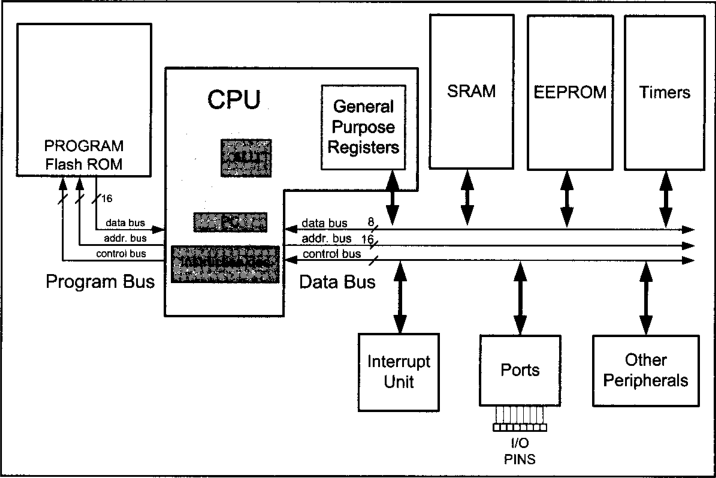
\includegraphics[scale=0.75]{./image/ARCHITECTURE/Harvard_architecture.png}\\
		\caption{Arquitetura Harvard}
		\label{Arquitetura Harvard}
	\end{figure}\par
	\end{comment}
	Os microcontroladores da AVR utiliza uma arquitetura de instru\c{c}\~{o}es {\bf RISC} (Reduced Instruction Set Computer ou Reduced COMPLEXITY Instruction Set Computer) na qual reduz a complexidade dos circuitos na codifica\c{c}\~{a}o de cada instru\c{c}\~{a}o. \par
	Dai que os microcontroladores que se baseiam nestes tipos de arquitetura s\~{a}o sinonimo de c\'{o}digo reduzido, alta performance e baixo consumo energ\'{e}tico \par
	\begin{comment}
	\begin{figure}[H]
		\centering
		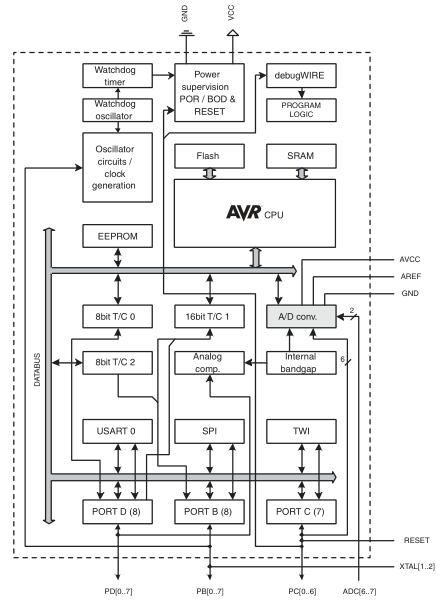
\includegraphics[scale=1]{./image/ARCHITECTURE/Block_diagram.png}\\
		\caption{Diagrama de blocos}
		\label{Diagrama de blocos}
	\end{figure}
	\end{comment}
%\newpage

	\section{Hardware}
	O micro-controlador a ser usado \'{e} um Atmega88, seu Datasheet (Manual do Componente) \'{e} uma pe\c{c}a fundamental para usar como suporte na sua utiliza\c{c}\~{a}o. \'{E} ligado uma ficha ISP aos respectivos pinos para programa\c{c}\~{a}o e debug. \\
	Para Facilitar seu desenvolvimento foi feito numa placa pre furada sua implementa\c{c}\~{a}o de forma a ser alimentada diretamente ao PC pela alimenta\c{c}\~{a}o da porta USB. \par
	Para programa\c{c}\~{a}o e debug do integrado \'{e} usado um Atmel-ICE, uma ferramenta de desenvolvimento que neste caso do i.c Atmega88 tem dispon\'{i}vel programa\c{c}\~{a}o via {\bf ISP} e debug por {\bf debugWIRE}. \\
	Os Par\^{a}metros de configura\c{c}\~{a}o do integrado s\~{a}o os seguintes, Device Signature do Atmega88=0x1E930A, {\bf ISP} clock a 1Mhz, BOOTZ=1024W\_0C00, SPIEN=ON, BODLEVEL=2V7, SUT\_CKSEL=EXTXOSC\_8MHZ\_XX\_16KCK\_14CK\_65MS , EXTENDED FUSE= 0xF9,HIGH FUSE=0xDD, LOW FUSE=0xFF com os restantes bits OFF. \\
	\begin{comment}	
	\begin{figure}[H]
		\centering
		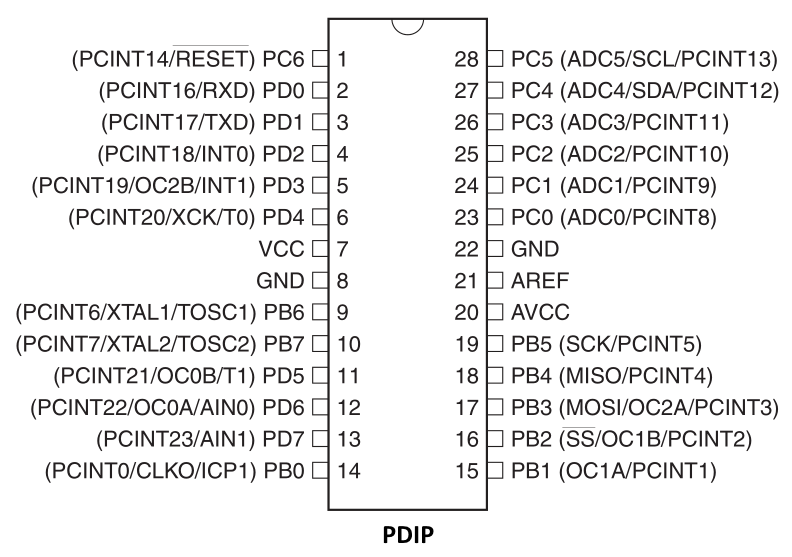
\includegraphics[scale=0.75]{./image/PACKAGE/Configuracao_pin.png}\\
		\caption{Configura\c{c}\~{a}o dos pinos}
	\end{figure}
	Para o programar foi ligado uma ficha ISP aos seus respectivos pinos. \\
	\begin{figure}[H]
		\centering
		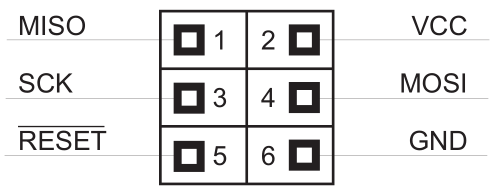
\includegraphics[scale=0.75]{./image/ISP_JTAG/isp_6pin.png}\\
		\caption{Ficha ISP}
	\end{figure}\par
	\end{comment}
%\newpage

	\section{Software}
	Nesta sec\c{c}\~{a}o \'{e} feito o c\'{o}digo correspondente em por um LED a piscar a 1Hz no PORTD6, nos casos mencionados na introdu\c{c}\~{a}o. \par
	A ferramenta de desenvolvimento ({\bf IDE}) utilizado \'{e} o Atmel Studio 6 (vers\~{a}o 6.2) \\
	Deve-se ter em aten\c{c}\~{a}o que no assembly a rotina JMP e CALL n\~{a}o funcionam no ATmega88 pois n\~{a}o fazem parte do seu conjunto de instru\c{c}\~{o}es, como indicado no seu Datasheet, mas recorrer a RJMP e RCALL respetivamente.	
	\begin{equation}
\boxed{F_{OCnx}=\frac{F_{clk\_I/O}}{2.N.(1+{OCRnx})}} \quad
\implies \quad {T_{OCRnx}=2.N.(1+OCRNx)\times T_{clk\_I/O}}
	\end{equation}

	\subsection{Led Pisca 1Hz em assembly por software.}
\begin{minipage}[T]{.3\linewidth}
.INCLUDE \textquotedblleft M88DEF.INC\textquotedblright \\
.ORG 0 \\
\hspace*{.5cm}	LDI R16, HIGH(RAMEND) \\
\hspace*{.5cm}	OUT SPH, R16 \\
\hspace*{.5cm}	LDI R16, LOW(RAMEND) \\
\hspace*{.5cm}	OUT SPL, R16 \\
\hspace*{.5cm}	LDI R16, (1$<<$6) \\
\hspace*{.5cm}	LDI R17, (1$<<$6) \\
\hspace*{.5cm}	SBI DDRD, 6 \\
BACK: \\
\hspace*{.5cm}	EOR R16, R17 \\
\hspace*{.5cm}	OUT PORTD, R16 \\
\hspace*{.5cm}	CALL DELAY\_ HalfSec \\
\hspace*{.5cm}	RJMP BACK \\
DELAY\_ HalfSec: \\
\hspace*{.5cm}	LDI R20, 32 \\
L1:	\hspace{.5cm} LDI R21, 100 \\
L2:	\hspace{.5cm} LDI R22, 250 \\
L3: \hspace{.5cm} \\
\hspace*{.5cm}	NOP \\
\hspace*{.5cm}	NOP \\
\hspace*{.5cm}	DEC R22 \\
\hspace*{.5cm}	BRNE L3 \\
\\
\hspace*{.5cm}	DEC R21 \\
\hspace*{.5cm}	BRNE L2 \\
\\
\hspace*{.5cm}	DEC R20 \\
\hspace*{.5cm}	BRNE L1 \\
\hspace*{.5cm}	RET \\[1ex]% [1ex] adds vertical space
;EOF \\
\end{minipage}
\qquad
\begin{minipage}[c]{.7\linewidth}
\begin{tikzpicture}[node distance = 2cm, auto]
% Define
\tikzstyle{RECTANGLE_1} = [rectangle, rounded corners, minimum width=1cm, minimum height=1cm,text centered, draw=black, fill=green!30]
\tikzstyle{RECTANGLE_2} = [rectangle, draw, align=left, fill=blue!20]
\tikzstyle{RECTANGLE_4} = [rectangle, draw, align=left, fill=orange!60]
\tikzstyle{RECTANGLE_3} = [rectangle, draw, align=left, fill=red!60]
\tikzstyle{DIAMOND_1} = [diamond, draw, align=left, fill=red!80]
\tikzstyle{ARROW} = [thick,->,>=stealth]
\tikzstyle{LINE} = [draw, -latex']
\tikzstyle{MYLINE} = [draw, ->,  thick, shorten <=4pt, shorten >=4pt]
% Place nodes
\node [RECTANGLE_1] (start) {.ORG 0};
\node [RECTANGLE_2, below of=start] (setup) {setup stack pointer\\ inicializar port};
\node [RECTANGLE_4, below of=setup] (TOGGLE) {TOGGLE LED};
\node [RECTANGLE_2, below of=TOGGLE] (R20) {R20=32};
\node [RECTANGLE_2, below of=R20] (R21) {R21=100};
\node [RECTANGLE_2, below of=R21] (R22) {R22=250};
\node [RECTANGLE_3, below of=R22] (DEC22) {DEC R22};
\node [DIAMOND_1, below of=DEC22] (BRNE22) {BRNE};
\node [RECTANGLE_3, left of=BRNE22,xshift=-.5cm] (DEC21) {DEC R21};
\node [DIAMOND_1, below of=DEC21] (BRNE21) {BRNE};
\node [RECTANGLE_3, left of=BRNE21,xshift=-.5cm] (DEC20) {DEC R20};
\node [DIAMOND_1, below of=DEC20] (BRNE20) {BRNE};
% LINES and ARROWS
\path [LINE] (start) -- node (l_1) {} (setup);
\path [LINE] (setup) -- node (l_2) {} (TOGGLE);
\path [LINE] (TOGGLE)-- node (l_3) {} (R20);
\path [LINE] (R20)-- node (l_4) {} (R21);
\path [LINE] (R21)-- node (l_5) {} (R22);
\path [LINE] (R21)-- node (l_5) {} (R22);
\path [LINE] (R22)-- node (l_6) {} (DEC22);
\path [LINE] (DEC22)-- node (l_7) {} (BRNE22);
\path [LINE] (BRNE22)-- node (l_8) {} (DEC21);
\path [LINE] (DEC21)-- node (l_9) {} (BRNE21);
\path [LINE] (BRNE21)-- node (l_10) {} (DEC20);
\path [LINE] (DEC20)-- node (l_11) {} (BRNE20);
\path [LINE] (BRNE20.east)|- +(+7,0) |- (l_4);
\path [LINE] (BRNE21.east)|- +(+4,0) |- (l_5);
\path [LINE] (BRNE22.east)|- +(+1,0) |- (l_6);
\path [LINE] (BRNE20.west)|- +(-.5,0) |- (l_2);
\end{tikzpicture}
\end{minipage}
\\
\\
\\
\\
Cada ciclo de maquina demora $1/8 Mhz$ que \'{e} igual a 125 nano segundos. \\
$Delay=32 \times 100 \times 250 \times 5 \times 125 ns \quad \implies \quad Delay=500ms$ \\
%;Neste calculo n\~{a}o esta inclu\'{i}do o atraso dos cabe\c{c}alhos dos dois ciclos exteriores.
%\newpage

	\subsection {Led pisca 1 Hz em C por Software.}	
\begin{minipage}[T]{.3\linewidth}
/***PreProcessor***/ \\
\#ifndef F\_CPU \\
\hspace*{.5cm}	\#define F\_CPU 8000000UL \\
\#endif \\
/***Library***/ \\
\#include \textless avr/io.h \textgreater \\
\#include \textless avr/interrupt.h \textgreater \\
\#include \textless util/delay.h \textgreater \\
\#include \textless avr/pgmspace.h \textgreater \\
/***Define and Macro***/ \\
\#define TRUE 1 \\
/***Global Variable***/ \\
/***Prototype***/ \\
void PORTINIT(void); \\
/***MAIN***/ \\
int main(void) \\
\textbraceleft \\
\hspace*{.5cm}	uint8\_t i,j,k; \\
\hspace*{.5cm}	PORTINIT(); \\
\hspace*{.5cm}    while(TRUE) \\
\hspace*{.5cm}    \textbraceleft \\
\hspace*{1cm}		for(i=32;i;i- -)\textbraceleft \\
\hspace*{1.5cm}			for(j=166;j;j- -)\textbraceleft \\
\hspace*{2cm}				for(k=250;k;k- -); \\
\hspace*{1.5cm}			\textbraceright \\
\hspace*{1cm}		\textbraceright \\
\hspace*{1cm}		PORTD\textasciicircum = (1$<<$PORTD6); \\
\hspace*{.5cm}	\textbraceright \\
\textbraceright \\
/***Procedure and Function***/ \\
void PORTINIT(void)\textbraceleft \\
\hspace*{.5cm}	DDRD=(1$<<$PORTD6); \\
\hspace*{.5cm}	PORTD=(1$<<$PORTD6); \\
\textbraceright \\
/***Interrupt***/ \\
/***EOF***/
\end{minipage}
\qquad
\begin{minipage}[c]{.7\linewidth}
\begin{tikzpicture}[node distance = 2cm, auto]
% Define
\tikzstyle{RECTANGLE_1} = [rectangle, rounded corners, minimum width=1cm, minimum height=1cm,text centered, draw=black, fill=green!30]
\tikzstyle{RECTANGLE_2} = [rectangle, draw, align=left, fill=blue!20]
\tikzstyle{RECTANGLE_11} = [rectangle, draw, align=left, fill=red!10]
\tikzstyle{RECTANGLE_12} = [rectangle, draw, align=left, fill=red!40]
\tikzstyle{RECTANGLE_13} = [rectangle, draw, align=left, fill=red!80]
\tikzstyle{RECTANGLE_3} = [rectangle, draw, align=left, fill=orange!60]
\tikzstyle{DIAMOND_1} = [diamond, draw, align=left, fill=red!10]
\tikzstyle{DIAMOND_2} = [diamond, draw, align=left, fill=red!40]
\tikzstyle{DIAMOND_3} = [diamond, draw, align=left, fill=red!80]
\tikzstyle{ARROW} = [thick,->,>=stealth]
\tikzstyle{LINE} = [draw, -latex']
\tikzstyle{MYLINE} = [draw, ->,  thick, shorten <=4pt, shorten >=4pt]
% Place nodes
\node [RECTANGLE_1] (start) {MAIN};
\node [RECTANGLE_2, below of=start] (setup) {uint8\_t i,j,k; \\ PORTINIT();};
\node [RECTANGLE_11, below of=setup] (for_1_inic) {i=32};
\node [DIAMOND_1, below of=for_1_inic] (for_1) {i==0};
\node [RECTANGLE_12, right of=for_1,xshift=.5cm] (for_2_inic) {j=166};
\node [RECTANGLE_3, left of=for_1,xshift=-1cm] (TOGGLE) {PORTD\textasciicircum \\ = (1$<<$PORTD6);};
\node [DIAMOND_2, below of=for_2_inic] (for_2) {j==0};
\node [RECTANGLE_13, right of=for_2,xshift=.5cm] (for_3_inic) {k=250};
\node [RECTANGLE_11, left of=for_2,xshift=-.5cm] (for_1_update) {i- -};
\node [DIAMOND_3, below of=for_3_inic] (for_3) {k==0};
\node [RECTANGLE_13, right of=for_3,xshift=.5cm] (for_3_update) {k- -};
\node [RECTANGLE_12, left of=for_3,xshift=-.5cm] (for_2_update) {j- -};
% LINES and ARROWS
\path [LINE] (start) -- node (l_1) {} (setup);
\path [LINE] (setup) -- node (l_2) {} (for_1_inic);
\path [LINE] (TOGGLE.west) |- +(-.1,0) |- (l_2);
\path [LINE] (for_1) -- node (l_11) {yes} (TOGGLE);
\path [LINE] (for_1) -- node (l_12) {no} (for_2_inic);
\path [LINE] (for_1_inic) -- node (l_10) {} (for_1);
\path [LINE] (for_1_update.west) |- +(-1,0) |- (l_10);
\path [LINE] (for_2_inic) -- node (l_21) {} (for_2);
\path [LINE] (for_2) -- node (l_20) {no} (for_3_inic);
\path [LINE] (for_2) -- node (l_22) {yes} (for_1_update);
\path [LINE] (for_2_update.west) |- +(-1,0) |- (l_21);
\path [LINE] (for_3_inic) -- node (l_30) {} (for_3);
\path [LINE] (for_3) -- node (l_31) {no} (for_3_update);
\path [LINE] (for_3) -- node (l_33) {yes} (for_2_update);
\path [LINE] (for_3_update) |- node (l_32) {} (l_30);
\end{tikzpicture}
\end{minipage}
\\
\\
\\
Os valores de i, j e k, foram do exerc\'{i}cio anterior que a posterior foi ajustado de forma a obter a frequ\^{e}ncia desejada, com o auxilio de um oscilosc\'{o}pio.
%\newpage

	\subsection {Led pisca 1 Hz em Assembly por Interrup\c{c}\~{a}o.}
\begin{minipage}[T]{.3\linewidth}
.EQU REPEAT = 100 \\
.EQU MASK = (1$<<$6) \\
.INCLUDE \textquotedblleft M88DEF.INC\textquotedblright \\[0.5ex]
.ORG 0 \\
\hspace*{.5cm}	RJMP RESET \\
.ORG 0x20 \\
\hspace*{.5cm}	RJMP TIM0\_COMPA \\
.ORG 0x100 \\
RESET: \\
\hspace*{.5cm}	LDI R16, HIGH(RAMEND) \\
\hspace*{.5cm}	OUT SPH, R16 \\
\hspace*{.5cm}	LDI R16, LOW(RAMEND) \\
\hspace*{.5cm}	OUT SPL, R16 \\
\hspace*{.5cm}	LDI R16, MASK \\
\hspace*{.5cm}	LDI R17, MASK \\
\hspace*{.5cm}	LDI R18, REPEAT \\
\hspace*{.5cm}	SBI DDRD, 6 \\
\hspace*{.5cm}	SBI PORTD, 6 \\
\hspace*{.5cm}	RCALL INTRUP\_10ms \\
\hspace*{.5cm}	RJMP MAIN \\
\hspace*{.5cm}	\\
; Setup Periodo 10ms \\
INTRUP\_10ms: \\
\hspace*{.5cm}	LDI R19, (1$<<$OCIE0A) \\
\hspace*{.5cm}	STS TIMSK0, R19 \\
\hspace*{.5cm}	LDI R19, 156 \\
\hspace*{.5cm}	OUT OCR0A, R19 \\
\hspace*{.5cm}	LDI R19, (1$<<$WGM01) \\
\hspace*{.5cm}	OUT TCCR0A, R19 \\
\hspace*{.5cm}	LDI R19, (1$<<$CS02) \\
\hspace*{.5cm}	OUT TCCR0B, R19 \\
\hspace*{.5cm}	SEI \\
\hspace*{.5cm}	\\
MAIN: \\
\hspace*{.5cm}	RJMP MAIN \\
\hspace*{.5cm}	\\
INIC: \\
\hspace*{.5cm}	LDI R18, REPEAT \\
\hspace*{.5cm}	EOR R16, R17 \\
\hspace*{.5cm}	
\hspace*{.5cm}	OUT PORTD, R16 \\
\hspace*{.5cm}	\\
TIM0\_COMPA: \\
\hspace*{.5cm}	DEC R18 \\
\hspace*{.5cm}	BREQ INIC \\
\hspace*{.5cm}	RETI \\
;EOF \\
\end{minipage}
\qquad
\begin{minipage}[c]{.7\linewidth}
\begin{tikzpicture}[node distance = 2cm, auto]
% Define
\tikzstyle{RECTANGLE_1} = [rectangle, align=left, rounded corners, minimum width=1cm, minimum height=1cm,text centered, draw=black, fill=green!30]
\tikzstyle{RECTANGLE_2} = [rectangle, draw, align=left, fill=blue!10]
\tikzstyle{RECTANGLE_3} = [rectangle, draw, align=left, fill=blue!40]
\tikzstyle{RECTANGLE_4} = [rectangle, draw, align=left, fill=purple!60]
\tikzstyle{RECTANGLE_5} = [rectangle, draw, fill=purple!60, text width=5em, text badly centered, minimum height=4em]
\tikzstyle{RECTANGLE_6} = [rectangle, draw, align=left, fill=red!60]
\tikzstyle{RECTANGLE_7} = [rectangle, draw, align=left, fill=orange!60]
\tikzstyle{DIAMOND_1} = [diamond, draw, align=left, fill=red!80]
\tikzstyle{ARROW} = [thick,->,>=stealth]
\tikzstyle{LINE} = [draw, -latex']
\tikzstyle{MYLINE} = [draw, ->,  thick, shorten <=4pt, shorten >=4pt]
% Place node
\node [RECTANGLE_1] (START) {.ORG 0x100};
\node [RECTANGLE_2, below of=START] (SETUP) {Setup Stack Pointer\\ Inicializar variaveis \\ Inicializar port};
\node [RECTANGLE_3, below of=SETUP] (INTERRUPT_SETUP) {Setup Interrupt \\ Parameters};
\node [RECTANGLE_5, below of=INTERRUPT_SETUP] (MAIN) {MAIN};
%
\node [RECTANGLE_1, below= 3cm of MAIN] (INTERRUPT_START) {.ORG 0x20 \\ (Interrupt Sequence)};
\node [RECTANGLE_6, below of=INTERRUPT_START] (DEC18) {DEC R18};
\node [DIAMOND_1, below of=DEC18] (BREQ18) {BREQ};
\node [RECTANGLE_6, right=1cm of BREQ18] (RETI) {RETURN TO MAIN};
\node [RECTANGLE_7, left=1cm of BREQ18] (INIC_COUNTER) {INIC COUNTER \\ (R18=100) \\ TOGGLE};
% LINES and ARROWS
\path [LINE] (START) -- node (l_1) {} (SETUP);
\path [LINE] (SETUP) -- node (l_2) {} (INTERRUPT_SETUP);
\path [LINE] (INTERRUPT_SETUP) -- node (l_3) {} (MAIN);
\path [LINE] (MAIN) |- ($(MAIN.south east) + (0.5,-0.5)$) |- (MAIN);
%
\path [LINE] (INTERRUPT_START) -- node (l_4) {} (DEC18);
\path [LINE] (DEC18) -- node (l_5) {} (BREQ18);
\path [LINE] (BREQ18) -- node (l_6) {no} (RETI);
\path [LINE] (BREQ18) -- node (l_7) {yes} (INIC_COUNTER);
\path [LINE] (INIC_COUNTER) |- ($(INIC_COUNTER.south east) + (5,-1)$) -- (RETI.south);
\end{tikzpicture}
\end{minipage} \\
\\
\\
\\
Usando Par\^{a}metros TIMSK0 com OCIE0A activado, wavegenmode=CTC, OCR0A=156 e por ultimo N=256, para obter um Per\'{i}odo de 10ms com oscila\c{c}\~{a}o por cristal $F_{clk\_I/O}=8Mhz$.

%\newpage

	\subsection {Led pisca 1 Hz em C por Interrup\c{c}\~{a}o.}
\begin{minipage}[T]{.3\linewidth}
/***PreProcessor***/ \\
\#ifndef F\_CPU \\
\hspace*{1cm} \#define F\_CPU 8000000UL \\
\#endif \\
/***Library***/ \\
\#include \textless avr/interrupt.h \textgreater \\
\#include \textless util/delay.h \textgreater \\
\#include \textless avr/io.h \textgreater \\
\#include \textless avr/pgmspace.h \textgreater \\
/***Define and macro***/ \\
\#define TRUE 1 \\
\#define REPEAT 100 \\
/***Global variable***/ \\
int count; \\
/***Prototype***/ \\
void PORTINIT(void); \\
void TIMER0ASETUP(void); \\
/***MAIN***/ \\
int main(void) \\
\textbraceleft \\
\hspace*{.5cm}	PORTINIT(); \\
\hspace*{.5cm}	TIMER0ASETUP(); \\
\hspace*{.5cm}	count = REPEAT; \\
\hspace*{.5cm}	while(TRUE) \\
\hspace*{.5cm}	\textbraceleft \\
\hspace*{1cm}   \\
\hspace*{.5cm}	\textbraceright \\
\textbraceright \\
/***Procedure and function***/ \\
void PORTINIT(void)\textbraceleft \\
\hspace*{.5cm}	DDRD = (1$<<$PORTD6); \\
\hspace*{.5cm}	PORTD = (1$<<$PORTD6); \\
\textbraceright \\
void TIMER0ASETUP(void)\textbraceleft \\
\hspace*{.5cm}	uint8\_{t} sreg; \\
\hspace*{.5cm}	sreg = SREG; \\
\hspace*{.5cm}	cli(); \\
/***Periodo de 10ms***/ \\
\hspace*{.5cm}	TCCR0A = (1$<<$WGM01); \\
\hspace*{.5cm}	TIMSK0 = (1$<<$OCIE0A); \\
\hspace*{.5cm}	OCR0A = 156; \\
\hspace*{.5cm}	TCCR0B \textbar = (1$<<$CS02); \\
\hspace*{.5cm}	SREG = sreg; \\
\hspace*{.5cm}	sei(); \\
\textbraceright \\
/***Interrupt***/ \\
ISR(TIMER0{\_}COMPA{\_}vect)\textbraceleft \\
\hspace*{.5cm}	count- -; \\
\hspace*{.5cm}	if(!count)\textbraceleft \\
\hspace*{1cm}		PORTD\textasciicircum = (1$<<$PORTD6); \\
\hspace*{1cm}		count = REPEAT; \\
\hspace*{.5cm}	\textbraceright \\
\textbraceright \\
/***EOF***/
\end{minipage}
\qquad
\begin{minipage}[c]{.7\linewidth}
\begin{tikzpicture}[node distance = 2cm, auto]
% Define
\tikzstyle{RECTANGLE_1} = [rectangle, align=left, rounded corners, minimum width=1cm, minimum height=1cm,text centered, draw=black, fill=green!30]
\tikzstyle{RECTANGLE_2} = [rectangle, draw, align=left, fill=blue!10]
\tikzstyle{RECTANGLE_3} = [rectangle, draw, align=left, fill=blue!40]
\tikzstyle{RECTANGLE_4} = [rectangle, draw, align=left, fill=purple!60]
\tikzstyle{RECTANGLE_5} = [rectangle, draw, fill=purple!60, text width=5em, text badly centered, minimum height=4em]
\tikzstyle{RECTANGLE_6} = [rectangle, draw, align=left, fill=red!60]
\tikzstyle{RECTANGLE_7} = [rectangle, draw, align=left, fill=orange!60]
\tikzstyle{DIAMOND_1} = [diamond, draw, align=left, fill=red!80]
\tikzstyle{ARROW} = [thick,->,>=stealth]
\tikzstyle{LINE} = [draw, -latex']
\tikzstyle{MYLINE} = [draw, ->,  thick, shorten <=4pt, shorten >=4pt]
% Place node
\node [RECTANGLE_1] (START) {MAIN};
\node [RECTANGLE_2, below of=START] (SETUP) {PORTINIT();\\ TIMER0ASETUP();\\ count=REPEAT;};
\node [RECTANGLE_5, below of=SETUP] (LOOP) {While Loop};%

\node [RECTANGLE_1, below= 3cm of LOOP] (INTERRUPT_START) {TIMER INTERRUPT ROUTINE};
\node [RECTANGLE_6, below of=INTERRUPT_START] (COUNT) {count- -};
\node [DIAMOND_1, below of=COUNT] (COUNTNULL) {!count};
\node [RECTANGLE_6, right=1cm of COUNTNULL] (RETURN) {RETURN};
\node [RECTANGLE_7, left=1cm of COUNTNULL] (INIC_COUNTER) {PORTD\^{}=(1$<<$PORTD6) \\ count=REPEAT;};
% LINES and ARROWS
\path [LINE] (START) -- node (l_1) {} (SETUP);
\path [LINE] (SETUP) -- node (l_2) {} (LOOP);
\path [LINE] (LOOP) |- ($(LOOP.south east) + (0.5,-0.5)$) |- (LOOP);
%
\path [LINE] (INTERRUPT_START) -- node (l_4) {} (COUNT);
\path [LINE] (COUNT) -- node (l_5) {} (COUNTNULL);
\path [LINE] (COUNTNULL) -- node (l_6) {no} (RETURN);
\path [LINE] (COUNTNULL) -- node (l_7) {yes} (INIC_COUNTER);
\path [LINE] (INIC_COUNTER) |- ($(INIC_COUNTER.south east) + (4,-1)$) -- (RETURN.south);
\end{tikzpicture}
\end{minipage} \\
\\
\\
$100 \times$ Periodo de 10ms $\implies$ 1sec de Periodo ou 1Hz
%\& \% \$ \# \_ \{ \} \textbackslash \textasciitilde \textasciicircum \textbackslash \par
%\newpage

	\section{Resultados}
	No geral foi conseguido os objetivos do relat\'{o}rio, o manuseamento e parametriza\c{c}\~{a}o do Atmega88 com o auxilio do datasheet \'{e} uma ferramenta importante, tendo tamb\'{e}m um bom debugger ajuda bastante no troubleshooting e dete\c{c}\~{a}o de problemas em conjunto com o Atmega Studio 6. 	
%\newpage

	\section{Conclus\~{o}es}
	O assembly \'{e} maquina dependente e de programa\c{c}\~{a}o detalhada muito ligada ao hardware, sua programa\c{c}\~{a}o em esparguete que n\~{a}o \'{e} aconselh\'{a}vel na linguagem C como por exemplo a instru\c{c}\~{a}o {\bf goto} em {\bf C}, da origem a c\'{o}digo dif\'{i}cil de seguir e se perceber.
	O {\bf C} \'{e} mais liberal maquina independente, mas o utilizador n\~{a}o tem controle sobre o mapeamento das avari\'{a}veis na memoria nem na sua compila\c{c}\~{a}o. A linguagem tamb\'{e}m \'{e} consebido com uma estrutura mais l\'{o}gica sendo sua transfer\^{e}ncia para {\bf Flowchart} mais intuitiva e fa\c{c}il. \par
	Fazendo {\bf Delays} ou {\bf Polling} interrompe o programa ficando a espera, dai as interrup\c{c}\~{o}es s\~{a}o mais \'{u}teis, s\'{o} chamando sua rotina quando necess\'{a}rio.
	
%%%%%%%%%%%%%%%%%%%%%%%%%%%%%%%%%%%%%%%%%%%%%%%%%%%%%%%%%%%%%%%%%%%%%%%%%%%%%%%%%%%%%%%%%%%%%%%%%%%
%%%%%%%%%%%%%%%%%%%%%%%%%%%%%%%%%%%%%%%%%%%%%%%%%%%%%%%%%%%%%%%%%%%%%%%%%%%%%%%%%%%%%%%%%%%%%%%%%%%
%%%%%%%%%%%%%%%%%%%%%%%%%%%%%%%%%%%%%%%%%%%%%%%%%%%%%%%%%%%%%%%%%%%%%%%%%%%%%%%%%%%%%%%%%%%%%%%%%%%
%%%%%%%%%%%%%%%%%%%%%%%%%%%%%%%%%%%%%%%%%%%%%%%%%%%%%%%%%%%%%%%%%%%%%%%%%%%%%%%%%%%%%%%%%%%%%%%%%%%
%%%%%%%%%%%%%%%%%%%%%%%%%%%%%%%%%%%%%%%%%%%%%%%%%%%%%%%%%%%%%%%%%%%%%%%%%%%%%%%%%%%%%%%%%%%%%%%%%%%
%%%%%%%%%%%%%%%%%%%%%%%%%%%%%%%%%%%%%%%%%%%%%%%%%%%%%%%%%%%%%%%%%%%%%%%%%%%%%%%%%%%%%%%%%%%%%%%%%%%
\newpage
\part*{Equa\c{c}\~{o}es} \label{eq}
%
\begin{flushleft}
{\bf Corrente Continua Condi\c{c}\~{o}es \index{Condi\c{c}\~{o}es} iniciais \index{iniciais} nulas \index{nulas}.}\par
\end{flushleft}
 \quad Circuito \index{Circuito} $LC$ em $C.C$:\par
%
\begin{itemize}
\item
$i(t)=\frac{V_{DC}\sqrt{LC}}{L}\quad \sin \left( \frac{t}{\sqrt{LC}}\right)\times u(t)$\par
\item
$V_L(t)=V_{DC}\quad \cos\left(\frac{t}{\sqrt{LC}} \right)\times u(t)$\par
\item
$V_c(t)=V_{DC}\quad \left(1-\cos\left(\frac{t}{\sqrt{LC}} \right) \right)\times u(t)$\par
\item
$\omega_n=\frac{1}{\sqrt{LC}}$\par
\item
$\overline{Z}=\sqrt{(\omega_n L-\frac{1}{\omega_n C})^2}$\par
\item
$\phi_p=\frac{\pi}{2}$\par
porque, $\sin(\omega_n t)= \cos(\omega_n t - \pi/2)$\par
\item
$\tau=\infty$\par
\end{itemize}
%
%%%%%%%%%%%%%%%%%%%%%
\quad Circuito \index{Circuito} $RLC$ em $C.C$:\par
%
\begin{enumerate}
%enum1
\item
Para \quad $C(C R^2-4 L)>0$ \quad (Ra\'{i}zes \index{Ra\'{i}zes} reais \index{reais} diferentes \index{diferentes}) \quad Sobreamortecido \index{Sobreamortecido}.\par
%
\begin{itemize}
\item
$i(t)=\frac{2 V_{DC} C e^{\frac{-tR}{2L}} sinh \left( \frac{t \sqrt{C(CR^2-4L)}}{2CL} \right)}{\sqrt{C(CR^2-RL)}}\times u(t)$\par
\item
$V_R(t)=R\times i(t)$\par
\item
$V_L(t)=L\dfrac{di(t)}{dt}$\par
%
\begin{minipage}{0.95\linewidth}
\makebox[\linewidth]{
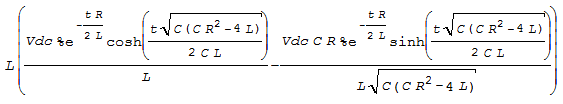
\includegraphics[scale=0.75]{./Image/equacoes_1.png}
}
\end{minipage}\par
%
\item
$V_C(t)=\frac{1}{C}\int_0^ti(t)$\par
%
\begin{minipage}{0.95\linewidth}
\makebox[\linewidth]{
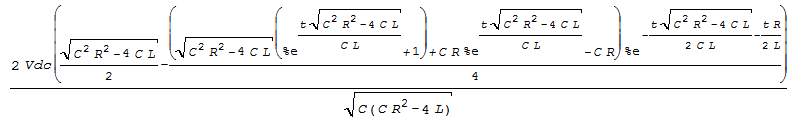
\includegraphics[scale=0.75]{./Image/equacoes_2.png}
}
\end{minipage}\par
%
\end{itemize}
%enum2
\item
Para \quad $C(C R^2-4 L)=0$ \quad (Ra\'{i}zes \index{Ra\'{i}zes} iguais \index{iguais})\quad Amortecimento \index{Amortecimento} cr\'{i}tico \index{cr\'{i}tico}.\par
%
\begin{itemize}
\item
$i(t)=\frac{V_{DC}}{L} \quad  t \quad e^{\frac{-R t}{2L}} \times u(t)$\par
\item
$V_R(t)=R\times i(t)$\par
\item
$V_L(t)=L\dfrac{di(t)}{dt}$\par
%
\begin{minipage}{0.95\linewidth}
\makebox[\linewidth]{
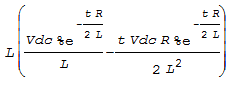
\includegraphics[scale=0.75]{./Image/equacoes_3.png}
}
\end{minipage}\par
%
\item
$V_C(t)=\frac{1}{C}\int_0^ti(t)$\par
\begin{minipage}{0.95\linewidth}
\makebox[\linewidth]{
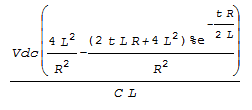
\includegraphics[scale=0.75]{./Image/equacoes_4.png}
}
\end{minipage}\par
%
\end{itemize}
%enum3
\item
Para \quad $C(C R^2-4 L)<0$ \quad (Ra\'{i}zes \index{Ra\'{i}zes} complexas \index{complexas}) \quad Amortecido \index{Amortecido}.\par
%
\begin{itemize}
\item
$i(t)=\frac{2 V_{DC} C e^{\frac{-tR}{2L}} sin \left( \frac{t \sqrt{-C(CR^2-4L)}}{2CL} \right)}{\sqrt{-C(CR^2-4L)}}\times u(t)$\par
\item
$V_R(t)=R\times i(t)$\par
\item
$V_L(t)=L\dfrac{di(t)}{dt}$\par
%
\begin{minipage}{0.95\linewidth}
\makebox[\linewidth]{
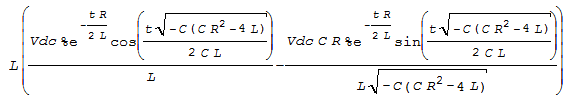
\includegraphics[scale=0.75]{./Image/equacoes_5.png}
}
\end{minipage}\par
%
\item
$V_C(t)=\frac{1}{C}\int_0^ti(t)$\par
%
\begin{minipage}{0.95\linewidth}
\makebox[\linewidth]{
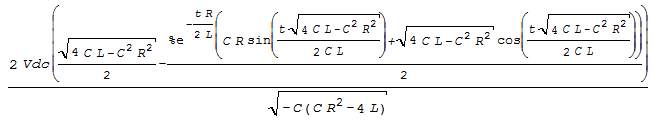
\includegraphics[scale=0.75]{./Image/equacoes_6.png}
}
\end{minipage}\par
%
\end{itemize}
\end{enumerate}
%
\begin{itemize}
\item
$| \omega_n |=\sqrt{\frac{4 L-R^2 C}{4 L^2 C}}$\par
\item
%\overrightarrow{Z}
$\overline{Z}=\sqrt{R^2 + (\omega_n L -\frac{1}{\omega_n C})^2}$\par
\item
$\phi_p=\arctan\left(\frac{\omega_n L - \frac{1}{\omega_n C}}{R}\right)$\par
\item
$\tau=\frac{2 L}{R}$\par
\end{itemize}
%%%%%%%%%%%%%%%%%%%%%%%%%%%%%%%%%%%%%%%%%%
\begin{flushleft}
{\bf Corrente \index{Corrente} Alternada condi\c{c}\~{o}es \index{Condi\c{c}\~{o}es} iniciais \index{iniciais} nulas \index{nulas}}.
\end{flushleft}
\quad Circuito \index{Circuito} $RLE$ em $C.A$:\par
\begin{itemize}
\item
$i(t)=C_T\ e^{-\frac{R}{L}t}+\frac{V_{m\acute{a}x}}{\overline{Z}}\sin(\omega t + \alpha - \phi_p)-\frac{E}{R}$\newline
$i(t)=C_T\ e^{-\frac{R}{L}t} + C_1 \cos (\omega t) + C_2 \sin(\omega t)-\frac{E}{R}$
\item
$I(\omega t)=C_T\ e^{-\frac{R}{L \omega}\omega t}+\frac{V_{m\acute{a}x}}{\overline{Z}}\sin(\omega t + \alpha - \phi_p)-\frac{E}{R}$
\item
$\overrightarrow{Z}=R+j\omega L$\\
$\overline{Z}=\sqrt{R^2 + (\omega L)^2}$
\item
$\phi_p=\arctan(\frac{\omega L}{R})$
\item
$C_T=\frac{E}{R}-\frac{V_{m\acute{a}x}}{\overline{Z}}\sin(\alpha - \phi_p)$
\item
$C_T=\frac{V_{m\acute{a}x}}{R^2 + (\omega L)^2}(L \omega \cos(\alpha) - R \sin (\alpha))+\frac{E}{R}$
\item
$C_1=\frac{V_{m\acute{a}x}}{R^2 + (\omega L)^2}(R \sin (\alpha) - L \omega \cos(\alpha))$
\item
$C_2=\frac{V_{m\acute{a}x}}{R^2 + (\omega L)^2}(R \cos (\alpha) + L \omega \sin (\alpha))$
%
\end{itemize}
%%%%%%%%%%%%%%%%%%%%%%%
%Figuras Bibliografia Index
%\newpage
%\listoffigures
%
\cite{*}
\bibliography{./bibliography/Bibliography}
%outro metodo mas manual\input{Bibliografia}
%
%\printindex
%
\newpage
\footnote{Apontamentos}
%
	\end{document}
%%%EOF%%%
